\documentclass[a4paper,11pt,pdftex, parskip]{scrreprt}
\usepackage[pdftex]{graphicx}
\usepackage{ngerman}
\usepackage[utf8]{inputenc}
\usepackage[T1]{fontenc}
\usepackage{lmodern}
\usepackage[numbers]{natbib}
\usepackage[margin=5pt,font=small,labelfont=bf, textfont=it]{caption}
%\usepackage[reals]{layout}
\usepackage[lmargin = 2cm, rmargin = 2cm, tmargin = 2cm]{geometry}
\usepackage{listings}
\lstset{language = Python, breaklines = true}
\lstset{numbers=left, numberstyle=\small, stepnumber=2, numbersep=8pt, frame=single, aboveskip= 10pt, belowskip=10pt}


\begin{document}
%\layout*
\begin{titlepage}

  
    \title{
        \begin{figure}[t]
            \centering
            
\includegraphics[scale = 0.125, keepaspectratio]{Logos/wwu_logo.png}
            \hspace{1cm}
            
\includegraphics[scale = 0.9, keepaspectratio]{Logos/ifgi_logo.png}
        \end{figure}
        % \begin{figure}[t]
        %     \centering
        %     \begin{minipage}[b]{.4\linewidth}
        %         
\includegraphics[scale = 0.1, angle = 0]{Logos/wwu_logo.png}
        %        \end{minipage}
        %     \begin{minipage}[b]{.5\linewidth}
        %      
\includegraphics[scale = 0.4, angle = 0 ]{Logos/ifgi_logo.png}
        %     \end{minipage}
          
        %    \end{figure}
           
        \textnormal{ 
            \normalsize \Large 
            Westfälische Wilhelms Universität \\ Institut für Geoinformatik\\
            \vspace{3cm}
           % \LARGE 
            Proposal zu\\}
        \glqq {Semantische Kompression von Drohnenvideos \\ mit der Discrete Curve Evolution}\grqq
        %Semantische Kompressino von Drohnenvideos mit der Discrete Curve Evolution 
        \vspace{1,5cm}}

   
    \author{ 
        Erstgutachter: Prof. Dr. Reinhard Moratz \\
        Zweitgutachter: Dr. Christian Knoth \\
        Ausgabetermin: tbd. \\
        \vspace{0.75cm}
        Abgabetermin: tbd. \\
        Vorgelegt von: Timo Lietmeyer \\
        Geboren am : 23.05.1999 \\
        E-Mail-Adresse: timolietmeyer@uni-muenster.de \\
        Matrikelnummer: 459 169 \\
        Studiengang: Bachelor Geoinformatik
    }
    \date{ }    
\end{titlepage}
\maketitle
%\tableofcontents

\section*{1 Motivation}
Drohnen mit Kameras verbreiten sich immer weiter in Deutschland, wodurch eine stabile Verbindung von Pilot zu Drohne von hoher Wichtigkeit ist \citep{Nehring2021}. \newline
Da bei der immer weiter voranschreitenden technischen Entwicklung abzusehen ist, dass die Kameraauflösung bei Drohnen weiter steigt \citep{futuretrends2017}, ist auch eine stärkere Kompression dieser Bilder und Videos nötig, um eine stabile Verbindung weiter zu gewährleisten. Diese Kompression kann semantisch erfolgen, indem nur das übertragen wird, was auch gewünscht ist, um noch geringere Datenraten zu ermöglichen. Außerdem ist das Erreichen einer höheren Reichweite bei der Funkverbindung sehr wünschenswert. \newline
Eine Vereinfachung des detektierten Objekts kann außerdem eine Anonymisierung ermöglichen, da nur das Übertragen wird, was auch übertragen werden soll. Ein konkreter Anwendungsfall könnte die Zählung von Personen sein, die durch die Discrete Curve Evolution anonymisiert wurden.\\
Im Rahmen dieser Bachelorarbeit soll beispielhaft eine Methode implementiert werden, die eine Kompression von Drohnenvideos ermöglicht.
% \begin{itemize}
%     \item Sequenzierung von Objekten kann für bessere (semantische) Kompression mithilfe der Discrete Curve Evaluation (DCE) benutzt werden 
%     \item bessere Reichweite, stabilere Funkverbindungen von Drohne zu Pilot 
%     \item Dadurch können auch private Drohnennutzer von besseren Bedingungen profitieren 
%     \item Knoth:
%         \item Konkreten Use Case anführen (nicht nur Bandbreite erhöhen): Nur das übertragen was auch gesehen werden soll
%         \item Anonymisierung von aufgezeichneten Personen
%         \item kein Problem mit Betreuung
%         \item Was passiert mit den komprimierten Daten? Werden die beim Empfänger wieder zurückentpackt?
% \end{itemize}

\section*{2 Methodik}{
Zum Testen wird Videomaterial bereitgestellt, welches im Rahmen der Bachelorarbeit analysiert und komprimiert wird (s. Abb. \ref{Scr_ges_Vid}). Ein beispielhafter Verlauf ist in Abb. \ref{Bsp_Dorr} zu sehen. \\
Als ersten Schritt müssen die zu erkennenden Objekte detektiert werden (s. Abb. \ref{Scr_detail_Obj}). Bei dem Beispielvideo ist dies durch die statische Kameraposition in Verbindung mit den sich bewegenden Objekten durch Bewegtsegmentierung der beiden Objekte oder mit anderen Bilderkennungsalgorithmen, wie YOLO (You Only Look Once), möglich \Citep{Plastiras2018}. Dies ermöglicht die kontextabhängige Weieterverarbeitung.\newline
Weitergehend müssen die detektierten Bildsegmente in eine Binärmaske umgewandelt werden, welche vereinfacht werden kann. Das Umwandeln der segementierten Bildausschnitte in eine Binärmaske kann mithilfe eines Schwellwertverfahrens, welches von Nobuyuki Otsu entwickelt wurde, erfolgen \citep{Otsu1979}. \\
Die weitere Vereinfachung des Polygons erfolgt dann mithilfe der Discrete Curve Evolution (DCE).
% \begin{figure}
%     \lstinputlisting[firstline=131, lastline=140]{../Code/DCE.py}
%      \caption[testpsei]{Programmcode zur Methode XY}
    
% \end{figure}

  
\begin{figure}[ht]
    \centering
    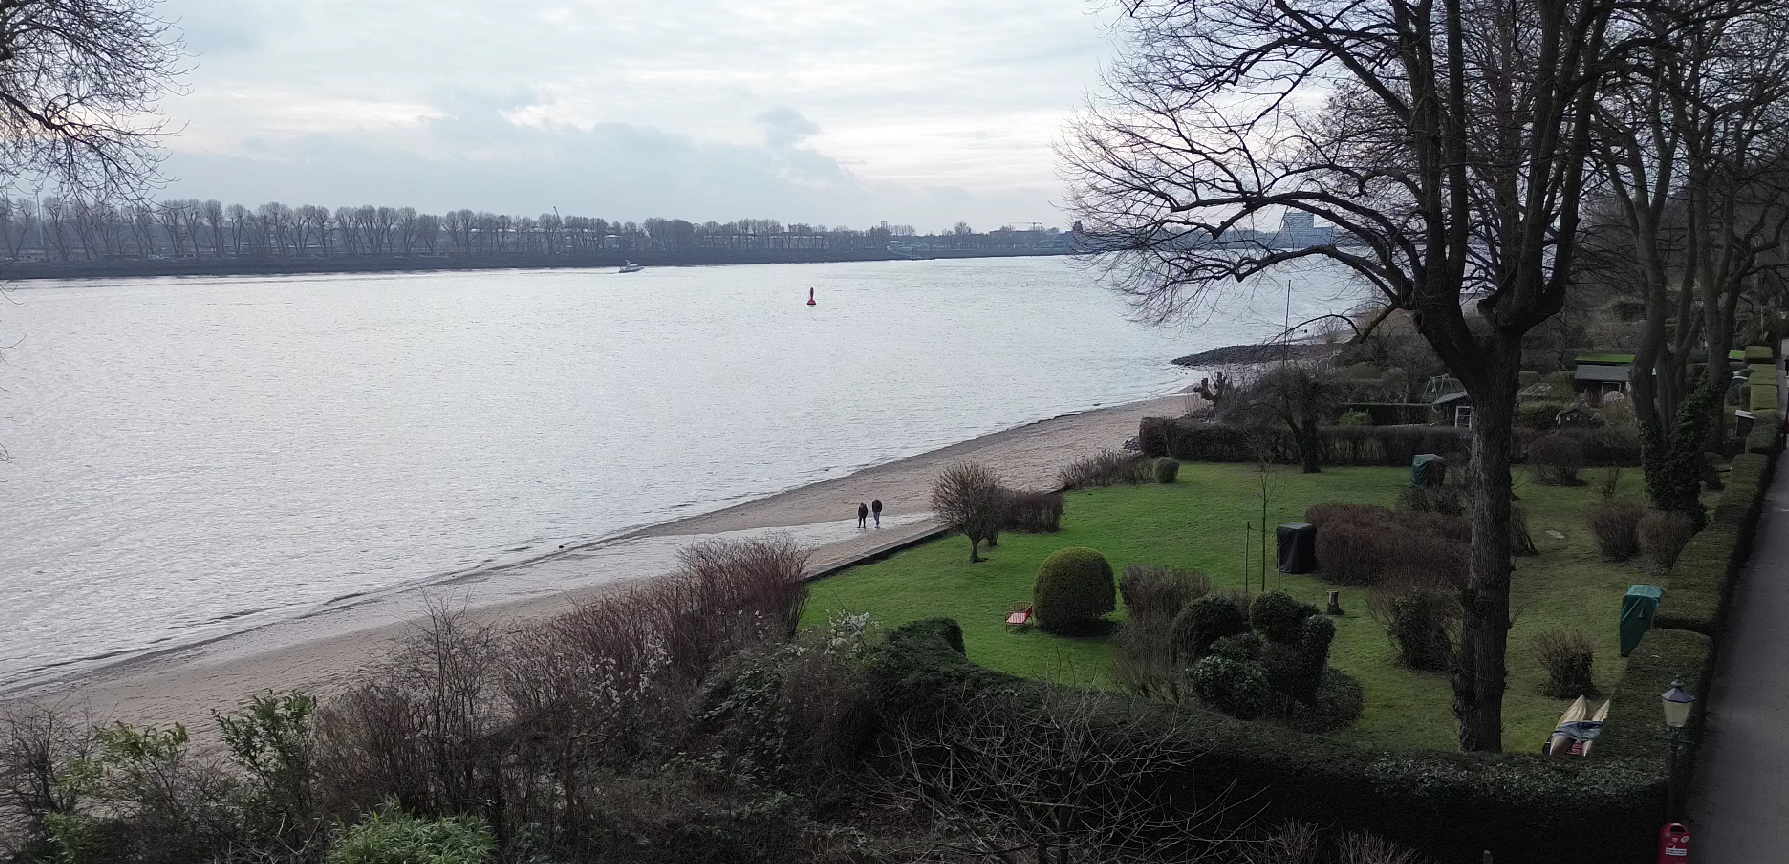
\includegraphics[scale=0.2, keepaspectratio]{images/screenshot_video_moratz.png}
    \caption[Screenshot des zu analysierenden Videos]{Screenshot des zu analysierenden Videos (Quelle: eigene Darstellung)}
    \label{Scr_ges_Vid}
\end{figure}
Diese berechnet anhand eines Grenzwertes, welche Punkte für die Darstellung einer Form irrelevant sind, sodass diese ohne größeren Informationsverlust entfernt werden können \citep{Barkowsky2000}. Durch die schrittweise Entfernung von Punkten kann eine bedarfsbezogene Vereinfachung des Polygons ermöglicht werden. \\
Anhand des komprimierten Videos, was als Ergebnis zu erwarten ist, kann eine Ergebnisevaluation stattfinden.
\begin{figure}[ht]
    \centering
    
\includegraphics[scale = 4, keepaspectratio] {images/detail_screenshot_people.png}
    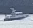
\includegraphics[scale = 4, keepaspectratio]{images/detail_screenshot_boat.png}
    \caption[Ausschnitte aus Abb. \ref{Scr_ges_Vid}, welche die beiden bewegenden Objekte darstellen ]{Ausschnitte aus Abb. \ref{Scr_ges_Vid}, welche die beiden bewegenden Objekte darstellen (Quelle: eigene Darstellung)}
    \label{Scr_detail_Obj}
\end{figure}
\begin{figure}[ht]
    \centering
    \includegraphics*[scale = 0.5, keepaspectratio]{images/Example_bird.png}
    \caption[Beispielablauf der Segmentierung und DCE aus \citet{Dorr2017}]{Beispiel, welches einen segementierten Vogel zeigt, der in eine Binärmaske umgewandelt wird. Dieses Polygon wird dann mithilfe der DCE vereinfacht (Quelle: \citep{Dorr2017})}
    \label{Bsp_Dorr}
\end{figure}
}


% \begin{itemize}
    
%     \item Anwendung von DCE und semantischer Kompression mithilfe von Bilderkennungsalgorithmen (Yolo, etc.)
%     \item Binärmaske aus segementierten Bildmaterial mit Hilfe von  Schwellwertverfahren von Nobuyuki Otsu (möglw.)
    

% \end{itemize}



% \section*{3 Evaluation}
% \begin{itemize}
%     \item Hier kommt ein Evaluationsstichpunkt
%     \item Anwendung auf von Betreuer zur Verfügung gestelltes Videomaterial
% \end{itemize}


\section*{3 Ausblick}
Wenn das Ergebnis der Komprimierung von Drohnenvideos mithilfe der DCE zufriedenstellend ist, kann eine hardwarenähere Programmierung erfolgen. Diese könnte in C oder C++ gemacht werden, um schnellere Ergebnisse liefern zu können, da die Prozessierungsgeschwindigkeit von Python begrenzt ist.\newline
Durch die hardwarenähere Implementierung der DCE könnte eine Komprimierung direkt am Aufzeichnungsort, bzw. in der Drohne, stattfinden, welche die Datenübertragungsrate senkt. Auch die Weiterentwicklung der integrierten Prozessoren in Drohnen ermöglicht möglicherweise in absehbarer Zeit vor Ort semantische Komprimierung mithilfe der DCE. Durch die Senkung der Datenübertragungsrate kann eine stabilere Funkverbindung, sowie höhere Reichweite ermöglicht werden.


% \begin{itemize}
%     \item Hier kommt ein Ausblickstichpunkt
%     \item Machbarkeitsstudie der DCE und semantischer Kompression auf Verbesserung der Verbindung zwischen Pilot und Drohne
%     \item Anwendung in C/C++, bzw. hardwarenaher umschreiben, damit schnellere (VorOrt-) Prozessierung/Kompression möglich ist
%     \item praktisches Beispiel entwicklen / eigene Drohnensoftware implementieren
% \end{itemize}

\appendix


\bibliographystyle{plainnat}
\bibliography{Bibliography}
\pagenumbering{roman}
\setcounter{page}{1}

\listoffigures



\end{document}